

%---------------------导言区---------------------------%
\documentclass[10pt,a4paper,twocolumn,twoside,UTF8]{ctexart}
	%10pt:正文字体为10pt,可以缺省;各层级字体大小会根据正文字体自动调整
	%a4paper:纸张大小a4;
	%twocolumn:双栏排版;
	%twoside:排版上分奇偶页,一般也就是有双面打印的需求;
	%UTF8:中文要求
\usepackage{geometry}%用于设置上下左右页边距
	%左右边距一样: 不考虑装订和翻页的需要.实验室网站上的示例论文格式报告就是这样。
	\geometry{left=2cm,right=2cm,top=2.5cm,bottom=4cm}
	%实际上,一般需要考虑到双面打印、装订和翻页的需要,需要区分奇偶页。奇偶页的页边距需要分开设置。奇数页左边距较宽,偶数页左边距较窄。
\usepackage{xeCJK,amsmath,paralist,enumerate,booktabs,multirow,graphicx,float,subfig,setspace,listings}
	%xeCJK:中文字体(如楷体,作者和机构需要用到)的设置
	%amsmath:数学公式
	%paralist,enumerate:自定义项目符号
	%booktabs:三线图,论文常用的表格风格
	%multirow:复杂表格
	%graphicx,float: 插入图片
	%subfig:并排排版图片以及强制图表显示在“这里”[H]
	%setspace:设置行间距等功能
	\setlength{\parindent}{2em}%正文首行缩进两个汉字
	%listings:用于排版各种代码;比如matlab的代码
	\lstset{language=c++}%matlab代码
	%代码环境的使用可以参考完整实验报告模板

\setCJKmainfont{FZShuSong-Z01S}[ItalicFont=FZKai-Z03S, BoldFont=FZHei-B01S]
%中文字体设置:使用开源字体方正书宋,方正楷体和方正黑体

\usepackage{titlesec}
	%改变section、subsection里面字体的样式。中文黑体,英文TNR。
	\newfontfamily\sectionef{Times New Roman}
	\setCJKfamilyfont{FZHeiTi}{FZHei-B01S}
	\newcommand{\sectioncf}{\CJKfamily{FZHeiTi}}
	\titleformat*{\section}{\large\bfseries\sectioncf\sectionef}
	\titleformat*{\subsection}{\normalsize\bfseries\sectioncf\sectionef}


\usepackage{fancyhdr}
	%fancyhdr:一个很强大的宏包,用于自定义设计页面风格并命名以供调用。



%%begin----------设置首页和正文不同的页眉页脚----------------%%

\usepackage{ifthen}%这个宏包提供逻辑判断命令
\newboolean{first}%引入布尔变量
\setboolean{first}{true}%将布尔变量设置为true
\pagestyle{fancy}

	%%% Step1 定义正文的页面风格
	%E表示偶数页,O表示奇数页;R、L、C代表文字居右、居左、居中排版
	%页码:保证在外侧, 奇数页分布在右边,偶数页分布在左边
	%页眉中间的内容也因奇偶页而不同
	%实验名称根据实际情况修改
	\fancypagestyle{maincontent}{
		\fancyhf{}  %清空页眉页脚设置
		\fancyfoot[EC, OC]{\thepage}
		\renewcommand\footrulewidth{0pt}
	}

	

%%end--------------设置首页和正文不同的页眉页脚-----------%%



%%begin-----------------参考文献-----------------------%%

\usepackage{hyperref}%超链接
\usepackage[hyperref=true,backend=biber,bibstyle=gb7714-2015,citestyle=numeric-comp,sorting=none,backref=true]{biblatex}
	%hyperref=true和backref=true表示为各个参考文献的引用处、及定理、定义、例子等的引用处都添加上超链接;
	%backend=biber:后端处理的程序为biber.exe
	%bibstyle:参考文献风格;每个期刊、组织要求不同
		%gb7714-2015是目前国内期刊通用的风格,称为gb标准风格
	%citestyle:引用风格;每个期刊、组织要求不同
	%sorting=none:按照参考文献在论文中出现的先后顺序排序。
	%**编译:biblatex与biber命令配合使用。xelatex-biber-xelatex-xelatex
\addbibresource{book.bib}
	%这里写上.bib文件的相对地址
	%每次实验引用的页数不同,需要手动改变

%%end-------------------参考文献-----------------------%%




%%%%%%%%%%%%%%%%%%%%%%%%%%%%%%%%%%%%%%%%%%%%%%%%%%%%%%%%%%
%%%%%%%%%%%%%%%%%%%%%%%%%正文开始%%%%%%%%%%%%%%%%%%%%%%%%%%
%%%%%%%%%%%%%%%%%%%%%%%%%%%%%%%%%%%%%%%%%%%%%%%%%%%%%%%%%%

\begin{document}

%\textbf是粗体 \Large是17pt
\title{\Large\songti{蚁群算法}}
\date{}%不显示日期

%%begin-------------------中文摘要-----------------------%%

%\author{\large\textit{李妍妍}$^{1}$\\ \normalsize{(1 \textit{广州大学 {} 计算机科学与网络工程学院,广东{} 广州 }510000)}}


\twocolumn[
	%twocolumn: 双栏article下的单栏摘要
	\begin{@twocolumnfalse}
	\maketitle  %标题和作者
  	\renewcommand{\abstractname} {} %不显示摘要名字
	\begin{abstract}
	\vspace{-7em}
	%vspace:调整垂直空白,可以自己调整;缩小abstract和center(以及maketitle)的间距
	%\noindent %备用:摘要无缩进
	\setlength{\tabcolsep}{10.mm}{
		\begin{tabular}{| l | l |}% 通过添加 | 来表示是否需要绘制竖线
		\hline  % 在表格最上方绘制横线
		研究生姓名:李妍妍& 学号:2112006029\\
		\hline  %在第一行和第二行之间绘制横线
		所在专业:网络空间安全专业& 研究生所在学院:计算机科学与网络工程学院\\
		\hline % 在表格最下方绘制横线
		递交课程老师姓名: 高鹰& 评分(百分制): \\
		\hline  %在第一行和第二行之间绘制横线
		课程名称:人工智能中的仿生优化算法& 评分教师签名:\\
		\hline  %在第一行和第二行之间绘制横线
		\end{tabular}
	}
	
       \vspace{3em}
	{\bf 摘{} 要:}
	{\small 蚁群算法是一种模拟昆虫王国中蚂蚁群体觅食行为的仿生优化算法,该算法采用了正反馈并行自催化机制,具有较强的鲁棒性、优良的分布式计算机制、易于与其他方法结合等优点, 在解决许多复杂优化问题方面展现出其优异的性能。本文介绍了蚁群算法的原理以及该算法的两种成功的变形,通过阅读本文,可以对蚁群算法及其发展有着清晰的认识。}
	\par%空的新行的高度。
	\textbf{关键词}: Stigmergy; 蚁群算法;  最大一最小蚂蚁系统;  蚁群系统
	\vspace{3em}
	\end{abstract}
	\end{@twocolumnfalse}
	
]

%%end-------------------中文摘要-----------------------%%

\pagestyle{maincontent}%第二页之后的页面风格:maincontent

%%begin----------------层级结构------------------------%%

%重点1:知道每一个层级的样式和怎么和后面的正文接上
%重点2:掌握各种换段的方法
%重点3:自定义的项目符号(宏包enumerate的用法)

\section{引 \quad 言}
	%%section:第一级,节	,1
	群体智能是一种相对较新的解决问题的方法,它从昆虫和其他动物的社会行为中获得灵感。特别是蚂蚁的出现,激发了许多方法和技术的发展,其中研究得最多、最成功的是通用优化技术——蚁群优化。\par
	蚁群优化算法(ACO)的灵感来自于一些蚂蚁的觅食行为。这些蚂蚁在地面上沉积信息素,以便标记出一些有利的路径,以便其他蚁群成员遵循。蚁群优化利用类似的机制来解决优化问题。 \par
	自上世纪90年代初第一个蚁群优化算法提出以来,蚁群算法就引起了越来越多的研究人员的关注,目前已有许多成功的应用。此外,大量的理论研究结果将为蚁群算法的进一步应用提供有益的指导。 \par
	本文的目的是介绍蚁群优化的基本原理和其一些变体。第一部分提供了算法来源的蚁群觅食背景信息。第二节介绍蚁群算法的数学模型。第三节研究算法的主要变体。第四部分是全文的总结。

	%%section后面的正文:自动换段,正常缩进
	%%PS:这里出现了引用。一般就是做个样子,在引言引一下参考文献就好了。不引用后面的参考文献打印不出来。\cite{shenhan2015}
	%%自然换段:\par

%\newpage
%换一栏,而不是换一页。换一页用\clearpage
\section{蚁群觅食背景信息}
	\subsection{Stigmergy}
Stigmergy是一个自组织的机制,该机制描述的了这样一种交流方式: 无数的个体以一个共同的环境为媒介而发生相互作用,其结果导致了环境的更新,这个新的环境又为这些个体提供了新的相互作用的平台,它决定了未来环境的演化方向。 \par
Stigmergy 区别于其他communication的两个主要特征如下:
	\begin{itemize}
		\item[$1)$] Stigmergy是一种间接、非象征性、受环境影响的交流形式,例如: 昆虫通过改变环境来交换信息。
		\item[$2)$] Stigmergy是局部的: 它只能被那些访问到它被释放地点的昆虫获得。
	\end{itemize}
 	\subsection{Stigmergy在蚁群中的体现}
	Stigmergy机制可以在蚁群中观察到。在许多蚂蚁物种中,进出食物源的蚂蚁会在地面上沉积一种叫做信息素的物质。其他蚂蚁察觉到信息素的存在,倾向于沿着信息素浓度较高的路径走。通过这种机制,蚂蚁能够以一种非常有效的方式将食物运送到它们的巢穴。如图1所示:
%%% 1 不跨栏单幅图
	% 图片的大小需要细细得调。需要掌握latex里面的长度单位和限制大小方法。
	\begin{figure}[htbp]
		\centering
		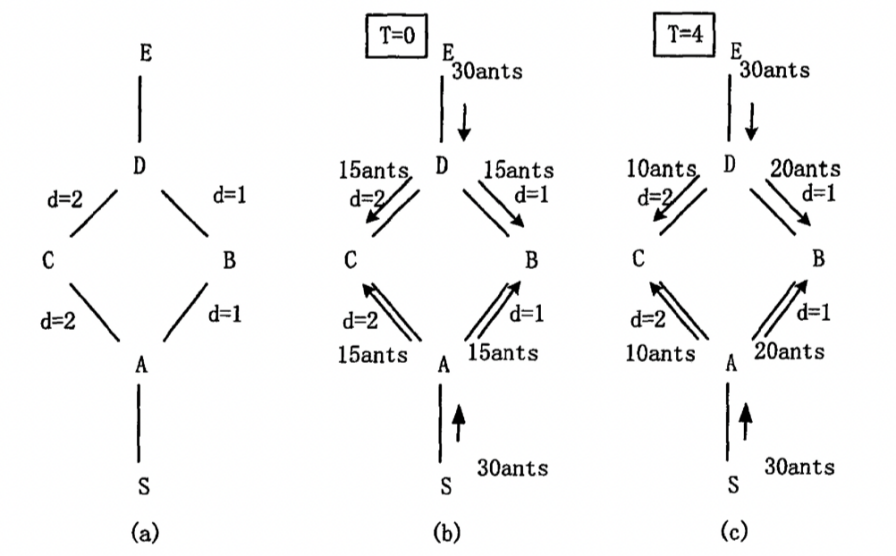
\includegraphics[width=0.3\textwidth]{img//pic1.png}
			%textwidth:正文宽度。双栏,则将两栏正文宽度相加。
		\caption{蚁群算法选择最短路径}
		\label{pic1}
	\end{figure}
	
	如图1,S,E两端各聚集有30只蚂蚁,运动速度相同,在T=0时,由于路径上没有信息素的累积,蚂蚁随机任意选择路径ABD或ACD,假设初始时每条路线分配一只蚂蚁,每个单位时间行走d=1,每经过一处留下信息素为1,则1个时间单位后,ABD上的蚂蚁到达终点时在ACD上的蚂蚁恰好完成路程的一半到达C点。T=4时,ABD路径的蚂蚁已完成2次往返,ACD路径上的只往返了一次,路径上的信息素值更新一次,两边比值为2:1。为了保证蚂蚁选择路径的合理性,规定蚂蚁只有完成一次往返后,才允许走选择过的路径。若寻找食物的过程继续进行,随着时间的推移,两条路线上蚂蚁的数量将会有显著的调整,大多数蚂蚁会根据信息素的指导选择ABD路径,ACD的较长路线上的蚂蚁将会越来越少,直至所有的妈蚁放弃ACD路线,S-A-B-D-E成为选择出的最优路径,蚁群实现了在两点间通过信息素协作机制选择最短路径的目的。

	\section{蚁群算法的数学模型}
	通过数学模型对蚁群算法进行详细阐述。
	\subsection{状态转移概率}
	蚂蚁k(k=1,2,3,...m)在运动过程中,会留下一定浓度的信息素,并通过判断各条路径上的信息素浓度$\gamma$确定其下一步的转移方向。用数学公式(1)表述在t时刻,处于位置点i的蚂蚁k选择下一步到达位置点j的概率$P_{ij}^k(t)$为:
		\begin{equation}
			P_{ij}^k(t)=
				\begin{cases}
				\frac{{\tau^ \alpha _{ij}(t) \eta ^ \beta _{ij}(t) }} {{\sum\limits_{S \subset allowed_k} [\tau^ \alpha_{is}(t) \eta^ \beta_{is}(t)] }}& \text{ $j \subset allowed_k$ }\\
				0& \text{others}
				\end{cases}
		\end{equation}	
	其中,$allowed_k = S-tabu_k(k=1,2,3...m)$表示蚂蚁k下一步可以选择的路径,列表$tabu_k$是为保证蚂蚁路线合理选择的设置的禁忌表,记录当前蚂蚁k未完成一次路径循环时途中所经过的所有路径,而当所有路径都被添加到$tabu_k$中时,说明结束了一次循环,而这条路径即成为所求问题解集中的一个解。A是代表残留信息素对蚂蚁的作用的信息素启发式因子:P代表蚂蚁k在运动过程中对信息素信息的重视程度,称为期望启发式因子,$\eta_{ij}(t)$被称为启发函数,定义见公式(2)
		\begin{equation}
		\eta_{ij}(t) = \frac{1}{d_{ij}}
		\end{equation}
	$d_{ij}$表示相邻路径i,j间的距离。蚁群算法中,对蚂蚁k来说,$d_{ij}$的值越小,$n_{ij}(t)$和$p_{ij}(t)$会相对増多,因此(2)式代表蚂蚁k从i向j转移的期望值。

	\subsection{信息素更新策略}
	当蚂蚁每次经过一个路径或完成了一次循环之后,会根据所走长度有适量地释放相应信息素,为了避免路径上之前残留的信息素会对启发信息产生干扰,而影响其他蚂蚁的判断,需要在每次的寻优过程中对信息素及时更新,各路径上的信息量使用公式(3)进行更新:
	\begin{equation}
		\tau_{ij}(t+1) = (1- \rho ) \tau_{ij}(t) + \Delta \tau_{ij}(t)   \rho\in (0,1)
	\end{equation}

式中, $\rho$为信息素的挥发系数,$1-\rho$则为信息素的保存系数;$\Delta \tau_{ij}(t)$表示此次循环路径上信息素的增量,可以表示公式(4)

	\begin{equation}
		\Delta\tau_{ij}(t) = \sum\limits^m_{k=1}\Delta\tau^k_{ij}(t)
	\end{equation}

式中,为蚂蚁k在此次循环中在路径(i,j)上释放的信息素量,若$tau_{ij}$=0,则代表该蚂蚁没有经过,初始时刻$tau_{ij}(0)$均为0

	\subsection{使用轮盘赌决定下一步路径}

通过各个个体的选择概率 ,计算其累计概率 。第k个个体的累计概率为$p_x(a_k) =  \sum\limits_{j=1}^k p_s(a_j)$。然后产生0到1之间的随机数e与$p_x(a_k)$进行比较来决定选择的个体 。若$a_{k-1}$则选择第 k 个个体。通过重复 n 轮来产生n个子代个体。

根据之前的状态转移概率公式计算出下一跳每一种可能的概率如表1所示:	
	 \begin{table}[H]
		\caption{\bf 各个类别的概率}
		\centering
		\begin{tabular}{|c|c|c|c| }% 通过添加 | 来表示是否需要绘制竖线
		\hline  % 在表格最上方绘制横线
		下一条选择路径& A & B & C \\
		\hline  %在第一行和第二行之间绘制横线
		概率& 0.76 & 0.19 & 0.05 \\
		\hline  %在第一行和第二行之间绘制横线
		\end{tabular}
	\end{table}
		
然后计算其累计概率,计算方法和结果如表2:
	\begin{table}[H]
		\caption{\bf 计算概率和}
		\centering
		\begin{tabular}{|c|c|c| }% 通过添加 | 来表示是否需要绘制竖线
		\hline  % 在表格最上方绘制横线
		A & B & C \\
		\hline  %在第一行和第二行之间绘制横线
		0.76+0.19+0.05=1 & 0.19+0.05=0.24 & 0.05 \\
		\hline  %在第一行和第二行之间绘制横线
		\end{tabular}
	\end{table}
接着生成一个0-1之间的随机数r,根据下面的公式来进行选择下一步的路径。
		\begin{equation}
			f(next) =
				\begin{cases}
				A& \text{ 0.24 <= r < 1 }\\
				B& \text{0.05 <= r < 0.24}  \\
				C& \text{0 <= r < 0.05}
				\end{cases}
		\end{equation}	
	
%%end------------------层级结构------------------------%%

%%begin------------------插入图表------------------------%%

\section{蚁群算法的两个优秀的变体}
	蚁群算法其本身当然也面临着一些不足,比如说搜索时间长,收敛速度慢,容易陷入局部最优解等问题。基于这些问题,Sttttzle和Hoss提出了最大一最小蚂蚁系统(MAX-MIN Ant System),该算法的主要 特点就是为信息素设置上下限来避免算法过早出现停滞现象; 还有基于对信息素矩阵进行局部和全局更新的蚁群系统(Ant Colony System) 。接下来就这两种优秀的变体进行详细的描述。为了好叙述问题,这里使用著名的旅行商问题。
	
	\subsection{MAX − MIN Ant System (MMAS)}
该算法是对原有蚁群算法的改进。它的特点是只有最好的蚂蚁更新信息素的浓度,信息素更新的实现如下:
	\begin{equation}
	\tau_{ij}\leftarrow\left[(1-\rho)\cdot\tau_{ij}+\Delta\tau_{i_{j}}^{{\rm best}}\right]_{\tau_{\min}}^{\tau_{\max}}
	\end{equation}	
式中,$\tau_{max}$和$\tau_{min}$分别为信息素的上界和下界;算子$[x]^a_b$定义为:
	\begin{equation}
	[x]_{b}^{a}=
		\begin{cases}
		a & \text{\rm if x > a, } \\
		b & \text{\rm if x < b,} \\ 
		x & \text{\rm otherwise;}
		\end{cases}
	\end{equation}	
并且 	$\Delta\tau_{ij}^{best}$的定义如下:
	\begin{equation}
	\Delta\tau_{ij}^{best}=
	\begin{cases}
	\frac{1}{L_{best}} & \text{ if (i,j) belongs to the best tour } \\ 
	0 & \text{ otherwise;}
	\end{cases}
	\end{equation}	
	$L_{best}$是最好的蚂蚁旅程的长度。这可能是(取决于算法设计者的决定)当前迭代中找到的最佳路径或自算法开始以来找到的最佳解决方案或者是这两者的组合。
	关于信息素值的下界和上界,即$\tau_{max}$和$\tau_{min}$,它们通常是通过经验获得的
	
	\subsection{Ant Colony System (ACS) }
	ACS最有趣的贡献是除了在构建过程结束时进行的信息素更新(称为离线信息素更新)之外,还引入了局部信息素更新。
	每一步构建完成后,所有蚂蚁进行局部信息素更新。每只蚂蚁只将它应用于所遍历的最后一条边:
	
	\begin{equation}
	\tau_{ij}=(1-\varphi)\cdot\tau_{ij}+\varphi\cdot\tau_{0}
	\end{equation}	
	其中$\varphi\in(0,1]$为信息素衰减系数,$\varphi_0$为信息素的初值。
	
	局部更新的主要目标是使后续蚂蚁在一次迭代中进行的搜索多样化:通过降低横向边上的信息素浓度,蚂蚁鼓励后续蚂蚁选择其他边,从而产生不同的解。这使得几只蚂蚁在一次迭代中产生相同的解的可能性更小。
	
	离线信息素更新,类似于MMAS,在每次迭代结束时只由一只蚂蚁应用,这只蚂蚁可以是迭代最好的,也可以是迄今为止最好的。然而,更新公式略有不同:
	\begin{equation}
	\tau_{ij}\leftarrow
	\begin{cases}
	(1-\rho) \cdot \tau_{ij} \cdot + \rho \cdot \Delta\tau_{ij} & \text{ if (i,j) belongs to best tour;} \\
	\tau_{ij} & \text{ otherwise; } 
	\end{cases}
	\end{equation}	
	
	对于$MMAS$, $\tau_{ij}= 1/L_{best} $,  $L_{best}$的取值也是要么是$L_{ib}$要么是$L_{bs}$
	
	ACS和AS的另一个重要区别是蚂蚁在建造过程中使用的决策规则。在ACS中使用了伪随机比例规则:一只蚂蚁从城市i到城市j的转移概率取决于一个均匀分布在[0,1]上的随机变量q,和参数$q_0$;如果$q\leq q_0$,然后 $j = arg max_{c_{il}\in N(s^p)} \{   \tau_{il}\eta_{il}^ \beta \} $。	
%%% 1 不跨栏单幅图
	% 图片的大小需要细细得调。需要掌握latex里面的长度单位和限制大小方法。	
\section{结束语}
	本文介绍了仿生优化算法中的一个重要的概念:Stigmergy以及其在蚁群算法中的体现。对于蚁群算法,通过旅行商问题,详细的介绍了其经典的算法,以及两个非常成功的改进算法。对于蚁群算法的数学模型和整个流程也给了详细的阐述,从而对蚁群算法有了更清晰的认识。
	
%%end--------------------插入公式------------------------%%
% 这里文献较不规范 先不使用bib
%\printbibliography[title=参考文献]%打印参考文献
	%title:默认是英文的reference,用这个选参数改成中文
	
	\begin{thebibliography}{99}  
		\bibitem{ref1} Dorigo M, Birattari M, Stutzle T. Ant colony optimization[J]. IEEE computational intelligence magazine, 2006, 1(4): 28-39.
		\bibitem{ref2}段海滨. 蚁群算法原理及其应用[M]. 科学出版社, 2005. 
		\bibitem{ref3}李擎, 张超, 陈鹏, 等. 一种基于粒子群参数优化的改进蚁群算法[D]. 东北大学, 2013. 
		\bibitem{ref4}Dorigo M, Blum C. Ant colony optimization theory: A survey[J].Theoretical computer science, 2005, 344(2-3): 243-278.
		\bibitem{ref5}Blum C. Ant colony optimization: Introduction and recent trends[J]. Physics of Life reviews, 2005, 2(4): 353-373.
		\bibitem{ref6}Wang J, Cao J, Sherratt R S, et al. An improved ant colony optimization-based approach with mobile sink for wireless sensor networks[J]. The Journal of Supercomputing, 2018, 74(12): 6633-6645.
		\bibitem{ref7}Xu X, Zhao Z, Li R, et al. Brain-inspired stigmergy learning[J]. IEEE Access, 2019, 7: 54410-54424.
		\bibitem{ref8}Mavrovouniotis M, Müller F M, Yang S. Ant colony optimization with local search for dynamic traveling salesman problems[J]. IEEE transactions on cybernetics, 2016, 47(7): 1743-1756.
	\end{thebibliography}


\end{document}
